\section{Conclusion and Discussion}
\label{sec:diss}
In this paper we proposed a modular approach for learning manipulation task from human demonstration. We discover the number of modules needed in a task by hierarchical clustering. From each cluster we use forward and inverse model pairs to model the motor control mechanism. The forward models predict the effect of the previous motor command, while the inverse models compute a motor command to bring the current state to a desired state. The statistical approach enables us to estimate the reliability of the inferences of each module under the current context. The final motor command is the sum of the weighted command from each module. With an object centric viewpoint, the learnt human internal models can be easily transfer to robot. Our experiment verifies that by this modular approach, the robot can automatically recognize the current task context and compute proper motor commands to accomplish a manipulation task, i.e. opening bottle caps.

%We contribute an experimental validation of this approach by learning the human strategy of opening bottle cap. This is a complex manipulation task as the friction between the contact surfaces involve extremely complicated physics. Without detail knowledge of tribology, human success to open many different bottle caps in daily life. We aim to learn this strategy by a modular approach. The human demonstrator demonstrated the task in seven different contexts and we group these demonstrates into three groups. Forward and inverse model pairs are learnt from each group for motor control.

% TODO: where is useful, where is not useful
Our approach is applicable to manipulation tasks that require adaptive control strategy. It has a few benefits compare to the pervasive methods for adaptive control, e.g. classic model identification adaptive control and reinforcement learning. By imitating the human behaviors, we do not need to derive the system dynamics nor the cost function of the tasks, which involve deep insight of the task and can be painstaking. The difficulty of modeling an adaptive strategy is further reduced by a modular approach: dividing the large state space into several subspaces, where the local strategies can be approximated more accurately. With this approach, we divide the the complex human strategy into a few modules, and combine them to generate contextized motor commands.

Our object centric approach is a practical approach for teaching a robot manipulation tasks that require proprioception. This allows human demonstrating the task with physical contact with the object, and hence have direct feedback from their own sensory system. We bypass the problem of direct mapping human movement to robot movement by expressing the strategy from an object centric viewpoint. This can largely benefit learning manipulation tasks such as impedance control task, as measuring human muscle impedance is hard while measuring the impedance of an object is more feasible.

We compute the final motor command by summing the output of each module. This makes an assumption that the state space is continuous. For tasks with discontinuous space, constraints have to be applied and the other control methods mentioned above are more applicable.

There are many promising directions of further studies of this work. The first is to apply this approach to other contact tasks and learn a more general human control strategy in handling the instability caused by friction.
%Clarify the fact here that you hardly analyze the effect of changing the cap size and the positioning of the fingers on the cap which is revealed in the tactile signature, and that this will be future work.
In this study, we focus on the control strategy of unscrewing the cap. We hardly analyze the effect of changing the cap size and the positioning of the fingers on the cap, which is revealed in the tactile signature. This analysis will be progressed in the future work to study task specific grasping strategy~\ref{dang2014semantic}.

To extend our approach to learn tasks involve multiple steps, one could also integrate it with task segmentation technique, to break down the task into atomic steps and recognize the steps needs modular approach. How does the number of modules change according to the tasks is another useful information to reason about.

%So far we have implement the approach with a task controlled in three dimensions and by three modules. How does the number of modules change according to the dimension of the task is another useful information to reason about.

In summary, tasks involve multiple phases or different contexts are hard to implement by a single model. Modular architecture is a practical approach for modeling these tasks. As manipulation usually involves multi-phase friction and multi-body interaction, learning manipulation tasks with a modular approach can simplify the modeling problem in a large extend.

\begin{figure}
  \centering
  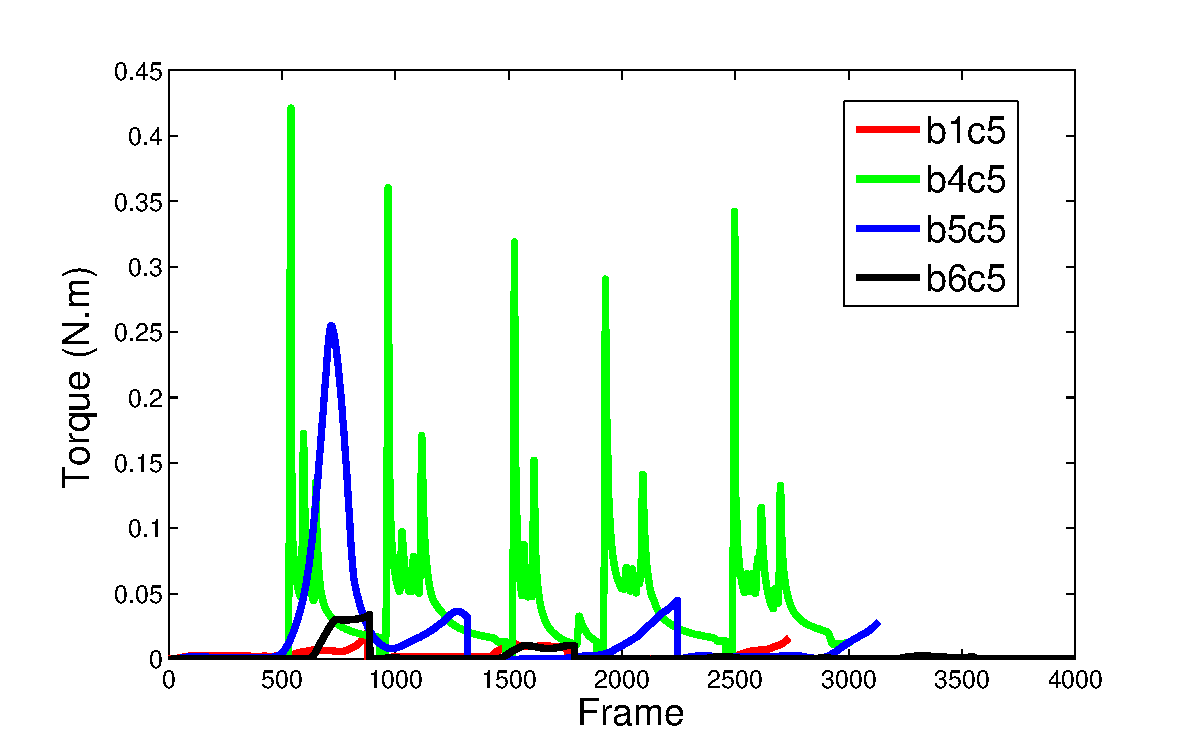
\includegraphics[width=8cm]{./fig/rb1b4b5b6_time_T.eps}
  \caption{ \scriptsize{Robot exert torque for opening four bottles: b1 b4 b5 b6. Time is warped and shifted for displace purpose.}
}
\label{fig:demo_b1b4b5b6}
\end{figure}

%\begin{itemize}
%  \item Can be used in more complex robot
%  \item if slip can be detected ...
%  \item grasp the cap, studied in another experiment
%\end{itemize}

%During the task, the dynamics of the environment changes abruptly. Figure~/ref{phase12} shows an example of the recorded time sequence of the opening bottle cap task. From the 4 turning cycles we see a dramatic difference between the first cycle and the rest of the cycles. This is not surprise as in the first turning cycle we have to apply a large torque to break the contact between the cap and the bottle, i.e. to overcome the static friction. Once the contact is broken, a much smaller torque is required to rotate the cap, i.e. to overcome the kinema.tic friction.
